\documentclass[12pt]{evanarticle}

\usepackage[columnsep=1cm, margin=1in]{geometry}

\addbibresource{~/cummings.evan@gmail.com/biblio.bib}

\begin{document}

\title{Computational Methods}

\author{Evan M.~Cummings}

\maketitle

\begin{abstract}
Basic linear interative methods are described and implemented in the computer language \texttt{C++}.
These methods are then used to solve three different systems of linear differential equations, and the convergence properties of each system are discussed.
\end{abstract}

%===============================================================================
%===============================================================================
\newpage
%===============================================================================
%===============================================================================

\section{Iterative methods} \label{sec_iterative_methods}

\begin{definition}[Basic iterative method] \label{def_basic_iterative_method}
Let $\ranktwo{A}$ be a $n \times n$ complex matrix.
We seek the solution $\rankone{x} \in \R^n$ of the linear system of equations
\begin{align}
	\label{linear_system}
	\ranktwo{A} \rankone{x} = \rankone{b}
\end{align}
for a given vector $\rankone{b} \in \R^n$.
To this end, split the matrix $\ranktwo{A}$ into \citep{varga_2000}
\begin{align*}
	\ranktwo{A} = \ranktwo{D} - \ranktwo{E} - \ranktwo{F},
\end{align*}
where $\ranktwo{D}$ is diagonal, $\ranktwo{E}$ is strictly lower triangular, and $\ranktwo{F}$ is strictly upper triangular.
Then system \cref{linear_system} is equivalent to
\begin{align*}
	\ranktwo{D}\rankone{x} = \left( \ranktwo{E} + \ranktwo{F} \right) \rankone{x} + \rankone{b},
\end{align*}
which suggests that an iterative method may defined as
\begin{align}
	\label{iterative_method}
	\ranktwo{D}\rankone{x}^{(m+1)} = \left( \ranktwo{E} + \ranktwo{F} \right) \rankone{x}^{(m)} + \rankone{b}
\end{align}
where $m \geq 0$.
In expanded form, \cref{iterative_method} is
\begin{align}
	\label{expanded_iterative_method}
	A_{ii} x_i^{(m+1)} = - \sum_{\substack{j=1 \\ j \not= i}}^n A_{ij} x_j^{(m)} + b_i.
\end{align}
where $1 \leq i \leq n$.
\end{definition}

%===============================================================================
%===============================================================================

\begin{definition}[Jacobi iteration] \label{def_jacobi}
Provided that the all the eigenvalues of $\ranktwo{A}$ are non-zero, the matrix $\ranktwo{D}$ is invertible.
Thus \cref{iterative_method} may be re-written as
\begin{align}
	\label{jacobi_interation}
	\rankone{x}^{(m+1)} = \ranktwo{D}^{-1} \left( \ranktwo{E} + \ranktwo{F} \right) \rankone{x}^{(m)} + \ranktwo{D}^{-1} \rankone{b},
\end{align}
or in expanded form as
\begin{align}
	\label{expanded_jacobi_iteration}
	x_i^{(m+1)} = - \sum_{\substack{j=1 \\ j \not= i}}^n \left( \frac{A_{ij}}{A_{ii}} \right) x_j^{(m)} + \frac{b_i}{A_{ii}}.
\end{align}
Relation \cref{expanded_jacobi_iteration} is referred to as \emph{Jacobi iteration}.
\end{definition}

%===============================================================================
%===============================================================================

\begin{definition}[Forward Gauss-Seidel iteration] \label{def_forward_gauss}
Observe that the sum from $j=1$ to $i-1$ of \cref{expanded_jacobi_iteration} can be computed using values of $x$ from the current iteration; \ie, splitting the matrices in \cref{iterative_method} into forward and backward parts produces
\begin{align}
	\label{forward_gauss_seidel_iteration}
	\ranktwo{D}\rankone{x}^{(m+1)} = \ranktwo{E}\rankone{x}^{(m+1)} + \ranktwo{F} \rankone{x}^{(m)} + \rankone{b},
\end{align}
so that
\begin{align}
	\label{forward_gauss_seidel_iteration_2}
	\rankone{x}^{(m+1)} = \left( \ranktwo{D} - \ranktwo{E} \right)^{-1} \ranktwo{F} \rankone{x}^{(m)} + \left( \ranktwo{D} - \ranktwo{E} \right)^{-1} \rankone{b}.
\end{align}
In expanded form, \cref{forward_gauss_seidel_iteration} is given by
\begin{align}
	\label{expanded_forward_gauss_seidel_iteration}
	x_i^{(m+1)} = - \sum_{j=1}^{i-1} \left( \frac{A_{ij}}{A_{ii}} \right) x_j^{(m+1)} - \sum_{j=i+1}^n \left( \frac{A_{ij}}{A_{ii}} \right) x_j^{(m)} + \frac{b_i}{A_{ii}}.
\end{align}
Observe that the inverse of $\ranktwo{D} - \ranktwo{E}$ is not required to be computed as the first sum in \cref{expanded_forward_gauss_seidel_iteration} does not require values of $x_j$ forward of $j$.
Hence relations \cref{forward_gauss_seidel_iteration} or \cref{expanded_forward_gauss_seidel_iteration} are referred to as the \emph{forward Gauss-Seidel iteration}.
\end{definition}

%===============================================================================
%===============================================================================

\begin{definition}[Backward Gauss-Seidel iteration] \label{def_backward_gauss}
Observe that the sum from $j=1$ to $i-1$ of \cref{expanded_jacobi_iteration} can be computed using values of $x$ from the current iteration; \ie, splitting the matrices in \cref{iterative_method} into forward and backward parts produces
\begin{align}
	\label{backward_gauss_seidel_iteration}
	\ranktwo{D}\rankone{x}^{(m+1)} = \ranktwo{E}\rankone{x}^{(m)} + \ranktwo{F} \rankone{x}^{(m+1)} + \rankone{b},
\end{align}
so that
\begin{align}
	\label{backward_gauss_seidel_iteration_2}
	\rankone{x}^{(m+1)} = \left( \ranktwo{D} - \ranktwo{F} \right)^{-1} \ranktwo{E} \rankone{x}^{(m)} + \left( \ranktwo{D} - \ranktwo{F} \right)^{-1} \rankone{b}.
\end{align}
In expanded form, \cref{backward_gauss_seidel_iteration} is given by
\begin{align}
	\label{expanded_backward_gauss_seidel_iteration}
	x_i^{(m+1)} = - \sum_{j=i-1}^{1} \left( \frac{A_{ij}}{A_{ii}} \right) x_j^{(m)} - \sum_{j=n}^{i+1} \left( \frac{A_{ij}}{A_{ii}} \right) x_j^{(m+1)} + \frac{b_i}{A_{ii}}.
\end{align}
Observe that the inverse of $\ranktwo{D} - \ranktwo{F}$ is not required to be computed as the second sum in \cref{expanded_backward_gauss_seidel_iteration} does not require values of $x_j$ backward of $j$.
Hence relations \cref{backward_gauss_seidel_iteration} or \cref{expanded_backward_gauss_seidel_iteration} are referred to as the \emph{backward Gauss-Seidel iteration}.
\end{definition}

%===============================================================================
%===============================================================================

\begin{definition}[Symmetric Gauss-Seidel iteration] \label{def_symmetric_gauss}
Consider a midpoint iteration $\rankone{x}^{(*)}$ of a Gauss-Seidel forward iteration
\begin{align*}
	\ranktwo{D}\rankone{x}^{(*)} = \ranktwo{E}\rankone{x}^{(*)} + \ranktwo{F} \rankone{x}^{(m)} + \rankone{b}
	\iff
	\rankone{x}^{(*)} = \left( \ranktwo{D} - \ranktwo{E} \right)^{-1} \ranktwo{F} \rankone{x}^{(m)} + \left( \ranktwo{D} - \ranktwo{E} \right)^{-1} \rankone{b}
\end{align*}
and backward iteration
\begin{align*}
	\ranktwo{D}\rankone{x}^{(m+1)} = \ranktwo{E}\rankone{x}^{(*)} + \ranktwo{F} \rankone{x}^{(m+1)} + \rankone{b}.
	\iff
	\rankone{x}^{(*)} = \ranktwo{E}^{-1} \left( \ranktwo{D} - \ranktwo{F} \right) \rankone{x}^{(m+1)} - \ranktwo{E}^{-1} \rankone{b}.
\end{align*}
Elimination of $\rankone{x}^{(*)}$ produces
\begin{align*}
	&&
	\ranktwo{E}^{-1} \left( \ranktwo{D} - \ranktwo{F} \right) \rankone{x}^{(m+1)} - \ranktwo{E}^{-1} \rankone{b}
	&= \left( \ranktwo{D} - \ranktwo{E} \right)^{-1} \ranktwo{F} \rankone{x}^{(m)} + \left( \ranktwo{D} - \ranktwo{E} \right)^{-1} \rankone{b} \\
	&\iff&
	\ranktwo{E}^{-1} \left( \ranktwo{D} - \ranktwo{F} \right) \rankone{x}^{(m+1)}
	&= \left( \ranktwo{D} - \ranktwo{E} \right)^{-1} \ranktwo{F} \rankone{x}^{(m)} + \left( \ranktwo{E}^{-1} + \left( \ranktwo{D} - \ranktwo{E} \right)^{-1} \right) \rankone{b} \\
	&\iff&
	\left( \ranktwo{D} - \ranktwo{F} \right) \rankone{x}^{(m+1)}
	&= \ranktwo{E} \left( \ranktwo{D} - \ranktwo{E} \right)^{-1} \ranktwo{F} \rankone{x}^{(m)} + \left( \ranktwo{\I} + \ranktwo{E} \left( \ranktwo{D} - \ranktwo{E} \right)^{-1} \right) \rankone{b}.
\end{align*}
Therefore,
\begin{align}
	\rankone{x}^{(m+1)}
	&= \left( \ranktwo{D} - \ranktwo{F} \right)^{-1} \ranktwo{E} \left( \ranktwo{D} - \ranktwo{E} \right)^{-1} \ranktwo{F} \rankone{x}^{(m)} + \left( \ranktwo{D} - \ranktwo{F} \right)^{-1} \left( \ranktwo{\I} + \ranktwo{E} \left( \ranktwo{D} - \ranktwo{E} \right)^{-1} \right) \rankone{b}.
\end{align}
However, the implementation avoids the calculations of any inverse matrices by instead calculating $\rankone{x}^{(*)} = \rankone{x}^{(m+1)}$ from forward iteration \cref{expanded_forward_gauss_seidel_iteration} which can then be used as a substitute for $\rankone{x}^{(*)} = \rankone{x}^{(m)}$ in backward iteration \cref{expanded_backward_gauss_seidel_iteration}.
\end{definition}

%===============================================================================
%===============================================================================

\begin{definition}[Richardson iteration] \label{def_richardson}
Observe that\footnote{Thanks to D.A.~Spielman (2009), \emph{Iterative solvers for linear equations}.}
\begin{align*}
	\ranktwo{A} \rankone{x} = \rankone{b}
	\iff
	\rankone{x} + \left( \ranktwo{A} - \ranktwo{\I} \right) \rankone{x} = \rankone{b}
	\iff
	\rankone{x} = \left( \ranktwo{\I} - \ranktwo{A} \right) \rankone{x} + \rankone{b}
\end{align*}
Hence an iterative method for $\rankone{x}$ is defined by
\begin{align}
	\label{richardson_iteration}
	\rankone{x}^{(m+1)} = \left( \ranktwo{\I} - \ranktwo{A} \right) \rankone{x}^{(m)} + \rankone{b},
\end{align}
or in expanded form as
\begin{align}
	\label{expanded_richardson_iteration}
	x_i^{(m+1)} = (1 - A_{ii}) x_i^{(m)} - \sum_{\substack{j=1 \\ j \not= i}}^n \left( A_{ij} \right) x_j^{(m)} + b_i.
\end{align}
Iteration \cref{richardson_iteration} is referred to as \emph{Richardson iteration}.
\end{definition}

%===============================================================================
%===============================================================================
\newpage
%===============================================================================
%===============================================================================

\section{Problem 1} \label{sec_problem_1}

Your task in this problem is to implement the three iterative methods we discussed in class for solving linear systems involving banded matrices.
Formally, consider an $n \times n$ matrix $\ranktwo{A}$ with entries $A_{ij}$.
If all matrix entries are zero outside a diagonally bordered band whose range is determined by constants $k_1, k_2 \geq 0$:
\begin{align*}
	A_{ij} = 0
	\hspace{5mm}
	\text{if}
	\hspace{5mm}
	j < i - k_1
	\hspace{5mm}
	\text{or}
	\hspace{5mm}
	j > i + k_2;
\end{align*}
then the quantities $k_1$ and $k_2$ are called the left- and right-half bandwidths, respectively.
The bandwidth of the matrix is defined as $b_w = k_1 + k_2 + 1$ (in other words, it is the smallest number of adjacent diagonals to which the non-zero elements are confined).
The functions should be declared as
\begin{cpp}
void <function_name>(int dim, int k1, int k2, vector<vector<double>> & A,
                   const vector<double> & b, vector<double> & x,
                   bool print_iter=false, int max_iter=1000,
                   double rtol=1.0e-7)
\end{cpp}
where \texttt{A} is the data containing the entries of the matrix $\ranktwo{A}$ that only stores the nonzero entries, \texttt{b} is the right hand side data vector, \texttt{x} is the vector to be calculated, \texttt{print\_iter} is a flag that if set will print iteration info, \texttt{max\_iter} is the maximum number of iterations allowed, and \texttt{rtol} is a small positive real number to be compared with	the relative residual
\begin{align*}
	\text{\texttt{relative\_residual}}
	= \frac{\norm{\rankone{\epsilon}^{(m)}}_2}{\norm{\rankone{\epsilon}^{(0)}}_2},
\end{align*}
where
$\rankone{\epsilon}^{(m)} = \rankone{b} - \ranktwo{A} \rankone{x}^{(m)}$
is the residual at iteration $m$.
Convergence is declared when \texttt{relative\_residual < rtol} or $m \geq$ \texttt{max\_iter}.
Here $\norm{ \cdot }_2$ is the usual Euclidean norm.

\begin{enumerate}

	\item Write a \texttt{C++} function \texttt{jacobi} that implements the Jacobi iteration.

	\item  Write a \texttt{C++} function \texttt{forwardGaussSeidel} that implements the forward Gauss-Seidel iteration.

	\item Write a \texttt{C++} function \texttt{symmetricGaussSeidel} that implements the symmetric Gauss-Seidel iteration, \ie, within one iteration perform one forward Gauss-Seidel and one backward Gauss-Seidel.

	\item Write a \texttt{C++} function \texttt{richardson} that implements the Richardson iteration.

\end{enumerate}

%===============================================================================
%===============================================================================

\subsection{Implementation} \label{sec_linear_implementation}

Since the matrix operations involved with this analysis do not involve inverting or transposing a matrix, the \emph{compressed row storage} representation of a sparse matrix is the most efficient method for calculating matrix-matrix and matrix-vector operations (\cref{matrix_header_code,matrix_code}).
The efficiency savings is clearly illustrated by the \texttt{EvanMatrix::dot} function of \cref{matrix_code}; instead of iterating over the $n^2$ operations associated with $n \times n$ matrix multiplication, it is only required to iterate over its non-zero entries.
Furthermore, the data for each operation is stored as a continuous block in main memory, and as such the processor can load data from main memory into cache as efficiently as possible.

The \texttt{linear\_solve} method (\cref{linear_header_code,linear_code}) utilizes the sparse matrix implementation just described and a parameter \texttt{method} which specifies which of the type of iterative method to use.
These are:
\begin{enumerate}

	\item \texttt{jacobi}: use Jacobi iteration \cref{def_jacobi}.

	\item \texttt{forwardGaussSeidel}: use forward Gauss-Seidel iteration \cref{def_forward_gauss}.

	\item \texttt{backwardGaussSeidel}: use backward Gauss-Seidel iteration \cref{def_backward_gauss}.

	\item \texttt{symmetricGaussSeidel}: use symmetric Gauss-Seidel iteration \cref{def_symmetric_gauss}.

	\item \texttt{richardson}: use Richardson iteration \cref{def_richardson}.

\end{enumerate}

A test script has been provided (\cref{test_code}) which may be used to test each of the implementations above.

%===============================================================================
%===============================================================================
\newpage
%===============================================================================
%===============================================================================

\subsection{Source code} \label{sec_1_source}

\cppexternal[label={matrix_header_code}, caption={C++ header file for sparse matrix implementation \cref{matrix_code}.}]{../src/evanmatrix.h}

\newpage

\cppexternal[label={matrix_code}, caption={C++ source code sparse matrix implementation used by \cref{linear_code} with corresponding header file given in \cref{matrix_header_code}.}]{../src/evanmatrix.cpp}

\newpage

\cppexternal[label={helper_header_code}, caption={C++ header file for a helper function with implementation \cref{helper_code}.}]{../src/helper.h}

\cppexternal[label={helper_code}, caption={C++ source code for helper functions.}]{../src/helper.cpp}

\newpage

\cppexternal[label={linear_header_code}, caption={C++ header file for linear solution methods with implementation \cref{linear_code}.}]{../src/linearSolver.h}

\newpage

\cppexternal[label={linear_code}, caption={C++ source code for the linear solution methods.}]{../src/linearSolver.cpp}

\newpage

\cppexternal[label={test_code}, caption={C++ source code test file used to create \cref{linear_code}.}]{../simulations/test.cpp}

%===============================================================================
%===============================================================================
\newpage
%===============================================================================
%===============================================================================

\section{Problem 2} \label{sec_problem_2}

Your task in this assignment is to calculate numerical solutions of two point boundary value problems (BVPs) using the iterative procedures in Problem 1.
Prior to doing this, we first need to develop a basic discretization technique of two point BVPs leading to a linear system governing the approximate solution.
Our benchmark problem is to approximate the solution for all $x \in (0,\ell)$ of
\begin{align}
	\label{ode}
	- \left( k(x) u'(x) \right)' &= f(x) \\
	\label{ode_0}
	u(0) &= u_0 \\
	\label{ode_l}
	-k(\ell) u'(\ell) &= g_{\ell}.
\end{align}
With the help of the fundamental theorem of calculus, integration of \cref{ode} over $(a,b)$, where $a,b \in (0,\ell)$ yields
\begin{align}
	\label{ode_int}
	k(a) u'(a) - k(b) u'(b)
	= \int_{a}^{b} f(x) \d{x} = \overline{f}_a.
\end{align}
We discretize $(0,\ell)$ into $n$ sub-intervals $(x_{i-1}, x_i)$ of length $h_i = x_i - x_{i-1}$ for $i = 1,2,\ldots,n$ such that $x_0 = 0$ and $x_n = \ell$.
We denote the midpoint of the interval $(x_{i-1}, x_i)$ by $m_i = x_{i-1} + h_i / 2$.
Observe that in particular, if $a = m_i$ and $b = m_{i+1}$ in \cref{ode_int}, then for $i = 1,2,\ldots,n-1$,
\begin{align}
	\label{ode_dis}
	k(m_i) u'(m_i) - k(m_{i+1}) u'(m_{i+1})
	= \int_{m_i}^{m_{i+1}} f(x) \d{x} = \overline{f}_i
\end{align}
We desire an approximate solution $\tilde{u}(x) \approx u(x)$ that is piecewise linear; \ie, for $i = 1,2,\ldots,n$,
\begin{align}
  \label{linear_approx}
  \tilde{u}(x)
	=
	\begin{cases}
		\tilde{u}_{i-1} + \left( \frac{\tilde{u}_i - \tilde{u}_{i-1}}{h_i} \right) (x - x_{i-1}), & x \in [x_{i-1}, x_i) \\
		0, & \text{otherwise}.
	\end{cases}
\end{align}
Putting it this way, we immediately see that $\tilde{u}(x_i) = \tilde{u}_i$ are the unknown coefficients at each node $i \in 0,1,2,\ldots,n$ of the discretization.
Also note that the derivative of linear approximation \cref{linear_approx} is
\begin{align}
  \label{linear_deriv_approx}
  \tilde{u}'(x)
	=
	\begin{cases}
		\frac{\tilde{u}_i - \tilde{u}_{i-1}}{h_i}, & x \in [x_{i-1}, x_i) \\
		0, & \text{otherwise}.
	\end{cases}
\end{align}
We further assume that the coefficient approximation $\tilde{k}(x) \approx k(x)$ in \cref{ode} is piecewise constant, \ie, for $i = 1,2,\ldots,n$,
\begin{align}
  \label{coef_approx}
	\tilde{k}(x)
	=
	\begin{cases}
		\tilde{k}_i, & x \in [x_{i-1}, x_i) \\
		0, & \text{otherwise}.
	\end{cases}
\end{align}
Insertion of approximations \cref{linear_deriv_approx,coef_approx} into \cref{ode_dis} produces
\begin{align*}
	\tilde{k}_i \left( \frac{\tilde{u}_i - \tilde{u}_{i-1}}{h_i} \right) - \tilde{k}_{i+1} \left( \frac{\tilde{u}_{i+1} - \tilde{u}_i}{h_{i+1}} \right)
	= \overline{f}_i,
\end{align*}
and isolation the coefficients $\tilde{u}_i$ gives
\begin{align}
	\label{system_1}
	\tilde{u}_{i-1} \left( -\frac{\tilde{k}_i}{h_i} \right) + \tilde{u}_i \left( \frac{\tilde{k}_i}{h_i} + \frac{\tilde{k}_{i+1}}{h_{i+1}} \right) + \tilde{u}_{i+1} \left( -\frac{\tilde{k}_{i+1}}{h_{i+1}} \right)
	= \overline{f}_i.
\end{align}
Relation \cref{system_1} represents a linear system of $n+1$ equations for $n+1$ coefficients $\tilde{u}_i$ which approximate the solution to \cref{ode,ode_0,ode_l}.
In compact form, this is equivalent to
\[ \ranktwo{K} \rankone{\coefvec{\tilde{u}}} = \rankone{\coefvec{b}},\]
where
$\rankone{\coefvec{\tilde{u}}} = \left[ \tilde{u}_0\ \tilde{u}_1\ \cdots\ \tilde{u}_n \right]^{\T} \in \R^{n+1}$,
$\rankone{\coefvec{b}} = \left[ \overline{f}_0\ \overline{f}_1\ \cdots\ \overline{f}_n \right]^{\T} \in \R^{n+1}$,
and the tri-diagonal coefficient matrix $\ranktwo{K} \in \R^{(n+1) \times (n+1)}$ is defined with components
\begin{align*}
	K_{ij}
	=
	\begin{cases}
		+ \frac{\tilde{k}_i}{h_i}, & j = i,\ i = 1 \\
		- \frac{\tilde{k}_i}{h_i}, & j = i + 1,\ i = 1 \\
		+ \frac{\tilde{k}_{i-1}}{h_{i-1}} + \frac{\tilde{k}_i}{h_i}, & j = i,\ 1 < i < n \\
		- \frac{\tilde{k}_{i-1}}{h_{i-1}}, & j = i - 1,\ 1 < i < n \\
		- \frac{\tilde{k}_i}{h_i}, & j = i + 1,\ 1 < i < n \\
		+ \frac{\tilde{k}_{i-1}}{h_{i-1}}, & j = i,\ i = n \\
		- \frac{\tilde{k}_{i-1}}{h_{i-1}}, & j = i -1,\ i = n \\
		+ 0, & \text{otherwise.}
	\end{cases}
\end{align*}

It remains to impose boundary conditions \cref{ode_0,ode_l}.
Observe that combining left boundary condition \cref{ode_0} with \cref{linear_approx} produces $\tilde{u}(0) = \tilde{u}_0 = u_0$.
Therefore, it is required that the system matrix satisfy the relation $\left[ \ranktwo{K} \rankone{\coefvec{\tilde{u}}} \right]_0 = u_0$; hence the first row of $\ranktwo{K}$ must be set to the first row of the identity matrix $\ranktwo{\I}$ and $\overline{f}_0 = u_0$.
At the right boundary, observe that if $a = m_n$ and $b = \ell$ in \cref{ode_int}, then
\begin{align*}
  k(m_n) u'(m_n) - k(\ell) u'(\ell)
  = \int_{m_n}^{\ell} f(x) \d{x} = \overline{f}_n
\end{align*}
and it follows from \cref{ode_l} that
\[
	k(m_n) u'(m_n) + g_{\ell} = \overline{f}_n;
\]
hence subtracting $g_{\ell}$ to both sides and applying \cref{linear_deriv_approx,coef_approx} produces
\begin{align*}
	\overline{f}_n - g_{\ell}
	= \tilde{k}_n \left( \frac{\tilde{u}_n - \tilde{u}_{n-1}}{h_n} \right)
	= \tilde{u}_{n-1} \left( \frac{ - \tilde{k}_n}{h_n} \right) + \tilde{u}_n \left( \frac{\tilde{k}_n}{h_n} \right)
	= \left[ \ranktwo{K} \rankone{\coefvec{\tilde{u}}} \right]_n;
\end{align*}
thus $g_{\ell}$ must be subtracted to the last element of the right-hand side vector $\rankone{\coefvec{b}}$.
Therefore, the matrix $\ranktwo{K}$ is transformed into
\begin{align*}
	K_{ij}
	=
	\begin{cases}
		+ 1, & j = i,\ i = 1 \\
		+ 0, & j = i + 1,\ i = 1 \\
		+ \frac{\tilde{k}_{i-1}}{h_{i-1}} + \frac{\tilde{k}_i}{h_i}, & j = i,\ 1 < i < n \\
		- \frac{\tilde{k}_{i-1}}{h_{i-1}}, & j = i - 1,\ 1 < i < n \\
		- \frac{\tilde{k}_i}{h_i}, & j = i + 1,\ 1 < i < n \\
		+ \frac{\tilde{k}_{i-1}}{h_{i-1}}, & j = i,\ i = n \\
		- \frac{\tilde{k}_{i-1}}{h_{i-1}}, & j = i -1,\ i = n \\
		+ 0, & \text{otherwise.}
	\end{cases}
\end{align*}
and the source vector is transformed into
$\rankone{\coefvec{b}} = \left[ u_0\ \overline{f}_1\ \cdots\ \overline{f}_n - g_{\ell} \right]^{\T} \in \R^{n+1}$.

\hrulefill

In all examples, use $\ell = 1$, $h_i = h = \ell/n$, and initial guess $\coefvec{\rankone{0}} \in \R^{n+1}$.
Try the following cases:
\begin{enumerate}
	\item $k(x) = 1$, $f(x) = 1$, $u_0 = 0$, and $g_{\ell} = 1$.
	\item $k(x) = 1$ if $0 < x < 0.5$ and $k(x) = 100$ if $0.5 \leq x < 1$, $f(x) = 0$, $u_0 = 0$, and $g_{\ell} = 1$.
	\item $k(x) = (1 - 0.95 \sin( 5 \pi x))^{-1}$, $f(x) = 1$, $u_0 = 1$, $g_{\ell} = 0$.
\end{enumerate}
Items to report:
\begin{enumerate}
	\item Plots of $n$ against number of iterations $m$ required to reach \texttt{relative\_residual < 1e-7}.
	Use $n = 10, 20, 40, 80, 160$.
	\item Plots of the solution against $x$ with comparison against the true solution.
	You may use $n = 20$ and $n = 160$.
	\item Give proper arguments and analysis of your results.
\end{enumerate}

%===============================================================================
%===============================================================================
\newpage
%===============================================================================
%===============================================================================

\subsection{Test cases}

\subsubsection{$\vect{k(x) = 1}$, $\vect{f(x) = 1}$, $\vect{u_0 = 0}$, and $\vect{g_{\ell} = -1}$} \label{sec_prob_2_part_a}

\begin{remark}
The flux $g_{\ell}$ has been made opposite in sign to that given in \cref{sec_problem_2} in order to generate a solution which is non-zero throughout its domain.
\end{remark}

\begin{claim} \label{claim_prob_2_part_1}
The general solution this problem is
$u(x) = 2x - \frac{1}{2} x^2.$
\end{claim}

\begin{proof}
Observe that ODE system \cref{ode,ode_0,ode_l} in this case is given by
\begin{align}
	\label{prob_2_part_1}
	- u''(x) = 1
	\hspace{5mm}
	u(0) = 0
	\hspace{5mm}
	u'(1) = 1
\end{align}
for all $x \in [0,1]$.
Thus integrating \cref{prob_2_part_1}$_1$ with respect to $x$ produces
\begin{align*}
	- \int u''(x) \d{x} = \int \d{x}
	\iff - u'(x) = x + C,
\end{align*}
which evaluated at $x = 1$ and applying \cref{prob_2_part_1}$_3$ is then
\begin{align*}
	-u'(1)
	= - 1
	= 1 + C
	\iff C = -2.
\end{align*}
Incorporating this and integrating once more with respect to $x$ gives
\begin{align*}
	- \int u'(x) \d{x} = \int ( x - 2 ) \d{x}
	\iff
	- u(x) = \frac{1}{2} x^2 - 2x + D,
\end{align*}
which after evaluation at $x = 0$ and applying \cref{prob_2_part_1}$_2$ becomes
\begin{align*}
	-u(0)
	= 0
	= D.
\end{align*}
Therefore, the general solution \cref{prob_2_part_1} is
\begin{align*}
	u(x) = 2x - \frac{1}{2} x^2,
\end{align*}
as expected.
\end{proof}

The exact solution and its approximation attained by applying forward-Gauss-Seidel iteration \cref{def_forward_gauss} are shown in \cref{fig_prob_2_part_a}.

\begin{figure}
	\centering
		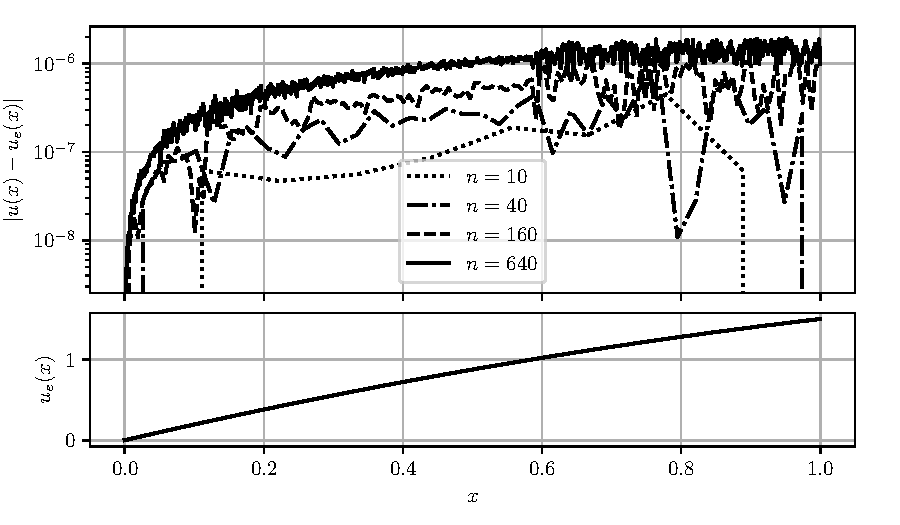
\includegraphics[width=1.0\linewidth]{../images/prob_2_part_a.pdf}
	\caption{The exact solution for \cref{claim_prob_2_part_1} (bottom axes) and the absolute error $| u(x) - u_e(x) |$ (top axes) for an indicated number of degrees of freedom $n$.
	The code used to generate this plot is given in Code \cref{plot_prob_a_code}.}
	\label{fig_prob_2_part_a}
\end{figure}

%===============================================================================
%===============================================================================
\newpage
%===============================================================================
%===============================================================================

\subsubsection{$\vect{k(x) = 1}$ if $\vect{0 < x < 0.5}$ and $\vect{k(x) = 100}$ if $\vect{0.5 \leq x < 1}$, $\vect{f(x) = 0}$, $\vect{u_0 = 0}$, and $\vect{g_{\ell} = -1}$.} \label{sec_prob_2_part_b}

\begin{remark}
The flux $g_{\ell}$ has been made opposite in sign to that given in \cref{sec_problem_2} in order to generate a solution which is non-zero throughout its domain.
\end{remark}

\begin{claim} \label{claim_prob_2_part_2}
The general solution to this problem is
\begin{align*}
	u(x)
	=
	\begin{cases}
	x, & x \in [0,0.5] \\
	\frac{x}{100} + \frac{99}{200}, & x \in [0.5, 1].
	\end{cases}
\end{align*}
\end{claim}

\begin{proof}
Observe that ODE system \cref{ode,ode_0,ode_l} in this case is given by
\begin{align}
	\label{prob_2_part_2}
	- (k(x) u'(x))' = 0
	\hspace{5mm}
	u(0) = 0
	\hspace{5mm}
	u'(1) = \frac{1}{100}
\end{align}
for all $x \in [0,1]$, where
\begin{align*}
	k(x)
	=
	\begin{cases}
		1, & 0 \leq x < 0.5 \\
		100, & 0.5 \leq x \leq 1.
	\end{cases}
\end{align*}
First, note that the solution $u_1$ restricted to the interval $0 \leq x < 0.5$ is determined using an identical process leading to \cref{claim_prob_2_part_1}.
Thus integrating \cref{prob_2_part_2}$_1$ with respect to $x$ with $k(x) = 1$ produces
\begin{align*}
	- \int u_1''(x) \d{x} = 0
	\iff u_1'(x) = C,
\end{align*}
which evaluated at $x = 0.5$ produces
$
	C = u_1'(0.5).
$
Incorporating this and integrating once more with respect to $x$ produces
\begin{align*}
	\int u_1'(x) \d{x} = \int u_1'(0.5) \d{x}
	\iff
	u_1(x) = u_1'(0.5) x + D,
\end{align*}
which evaluated at $x = 0$ and applying \cref{prob_2_part_2}$_2$ produces
$
	D = 0,
$
Therefore, the particular solution for $x \in [0,0.5]$ is
\begin{align}
	\label{prob_2_sol_1}
	u_1(x) &= u_1'(0.5)x.
\end{align}

Next, integrate \cref{prob_2_part_2}$_1$ with respect to $x$ with $k(x) = 100$:
\begin{align*}
	- 100 \int u_2''(x) \d{x} = 0
	\iff 100 u_2'(x) = C
\end{align*}
for some constant $C$, which evaluated at $x = 1$ and applying \cref{prob_2_part_2}$_3$ produces
$
	C = 1,
$
and therefore
\begin{align}
	\label{prob_2_part_sol_2_derivative}
	u_2'(x) = \frac{1}{100}.
\end{align}
Integrating once more with respect to $x$ produces
\begin{align*}
	\int u_2'(x) \d{x} = \frac{1}{100} \int \d{x}
	\iff
	u_2(x) = \frac{x}{100} + D
\end{align*}
for some constant $D$, which evaluated at $x = 0.5$ produces
\begin{align*}
	u_2(0.5) = \frac{1}{200} + D
	\iff
	D = u_2(0.5) - \frac{1}{200}
\end{align*}
Therefore, the particular solution for $x \in [0.5,1]$ is
\begin{align}
	\label{prob_2_sol_2}
	u_2(x) = 100 x + u_2(0.5) - \frac{1}{200}.
\end{align}

Next, the solution must be continuous such that $u_2(0.5) = u_1(0.5)$; thus evaluating \cref{prob_2_sol_1} at $x = 0.5$ produces
\begin{align}
	\label{prob_2_cont_u}
	u_2(0.5)
	= u_1(0.5)
	= \frac{u_1'(0.5)}{2}
\end{align}
Furthermore, the flux from the solution $u_1$ into the domain of the $u_2$ evaluated at the interface at $x = 0.5$ must also be equal; \ie,
\[ k(0.5) u_1'(0.5) = u_1'(0.5) = k(0.5) u_2'(0.5) = 100 u_2'(0.5). \]
Hence $u_1'(0.5) = 100 u_2'(0.5)$; this combined with \cref{prob_2_part_sol_2_derivative} produces
\begin{align}
	\label{prob_2_interface_flux}
	u_1'(0.5) = 100 u_2'(0.5) = \frac{100}{100} = 1
\end{align}
thus \cref{prob_2_interface_flux} transforms \cref{prob_2_cont_u} into
\begin{align}
	\label{prob_2_cont_u_deriv}
	u_2(0.5)
	= 0.5
\end{align}
Finally, combining \cref{prob_2_interface_flux} with \cref{prob_2_sol_1} produces
\begin{align}
	\label{prob_2_gen_sol_1}
	u_1(x) &= x.
\end{align}
for $x \in [0,0.5]$, and combining \cref{prob_2_cont_u_deriv} with \cref{prob_2_sol_2} produces
\begin{align}
	\label{prob_2_gen_sol_2}
	u_2(x) = \frac{x}{100} + \frac{99}{200}
\end{align}
for $x \in [0.5, 1]$.
\end{proof}

The exact solution and its approximation attained by applying forward-Gauss-Seidel iteration \cref{def_forward_gauss} are shown in \cref{fig_prob_2_part_b}.

\begin{figure}
	\centering
		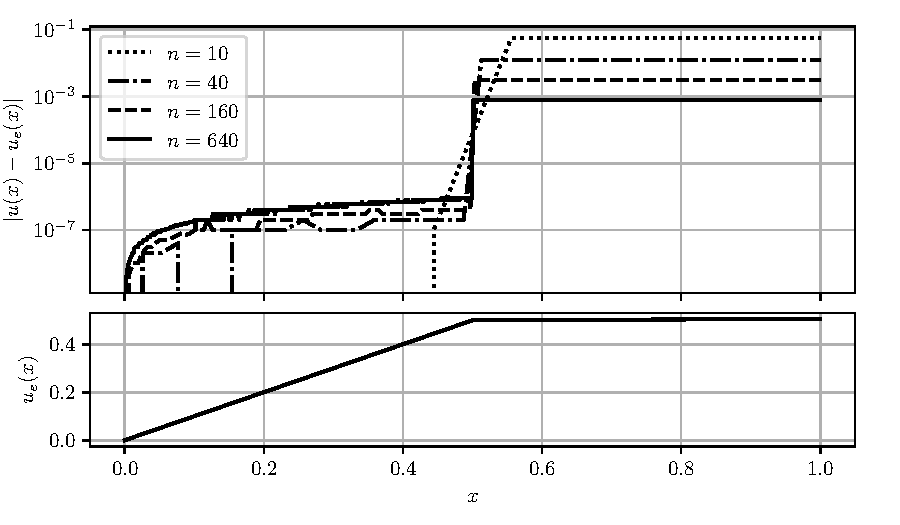
\includegraphics[width=1.0\linewidth]{../images/prob_2_part_b.pdf}
	\caption{The exact solution for \cref{claim_prob_2_part_2} (bottom axes) and the absolute error $| u(x) - u_e(x) |$ (top axes) for an indicated number of degrees of freedom $n$.
	The code used to generate this plot is given in Code \cref{plot_prob_b_code}.}
	\label{fig_prob_2_part_b}
\end{figure}

%===============================================================================
%===============================================================================
\newpage
%===============================================================================
%===============================================================================

\subsubsection{$\vect{k(x) = (1 - 0.95 \sin( 5 \pi x))^{-1}}$, $\vect{f(x) = 1}$, $\vect{u_0 = 1}$, $\vect{g_{\ell} = 0}$.} \label{sec_prob_2_part_c}

\begin{claim} \label{claim_prob_2_part_3}
The general solution to this problem is
\begin{align*}
	u(x)
	&= - \frac{x^2}{2} + x + \frac{19 \cos(5 \pi x)}{100 \pi} (1 - x) + \frac{19 \sin(5 \pi x)}{500 \pi^2} + \frac{100 \pi - 19}{100 \pi}.
\end{align*}
\end{claim}

\begin{proof}
Observe that ODE system \cref{ode,ode_0,ode_l} in this case is given by
\begin{align}
	\label{prob_2_part_3}
	- \totder{}{x} \left( k(x) \totder{u}{x} \right) = 1
	\hspace{5mm}
	u(0) = 1
	\hspace{5mm}
	\left. k(1) \totder{u}{x} \right|_{x = 1} = 0
\end{align}
for all $x \in [0,1]$, where
\begin{align*}
	k(x)
	= (1 - 0.95 \sin( 5 \pi x))^{-1}.
\end{align*}
Integrating both sides of \cref{prob_2_part_3}$_1$ with respect to $x$ yields
\begin{align*}
	-k(x) \totder{u}{x} = x + C
\end{align*}
for some constant $C$.
Evaluating this expression at $x = 1$ and applying \cref{prob_2_part_3}$_3$ implies that $C = -1$.
Therefore, dividing both sides of the resulting expression by $-k(x)$ gives
\begin{align*}
	\totder{u}{x} = \frac{1 - x}{k(x)}
	= (1 - x) \left(1 - \frac{19}{20} \sin( 5 \pi x) \right)
\end{align*}
combined with integrating once more with respect to $x$ yields
\begin{align*}
	u(x)
	&= \int (1 - x) \left(1 - \frac{19}{20} \sin( 5 \pi x) \right) \d{x} + D \\
	&= \int \left(1 - \frac{19}{20} \sin( 5 \pi x) \right) \d{x} - \int x \left(1 - \frac{19}{20} \sin( 5 \pi x) \right) \d{x} + D \\
	&= \left( x + \frac{19 \cos(5 \pi x)}{100 \pi} \right) - \left( \frac{x^2}{2} + \frac{19 x \cos(5 \pi x)}{100 \pi} - \frac{19 \sin(5 \pi x)}{500 \pi^2} \right)  + D
\end{align*}
for some constant $D$.
Finally, evaluating this expression at $x = 0$ and applying \cref{prob_2_part_3}$_2$ implies that
\begin{align*}
	1 = \frac{19}{100 \pi} + D
	\iff
	D = 1 - \frac{19}{100 \pi}
\end{align*}
Therefore, the general solution to \cref{prob_2_part_3} is
\begin{align*}
	u(x)
	&= \left( x + \frac{19 \cos(5 \pi x)}{100 \pi} \right) - \left( \frac{x^2}{2} + \frac{19 x \cos(5 \pi x)}{100 \pi} - \frac{19 \sin(5 \pi x)}{500 \pi^2} \right) + 1 - \frac{19}{100 \pi} \\
	&= - \frac{x^2}{2} + x + \frac{19 \cos(5 \pi x)}{100 \pi} (1 - x) + \frac{19 \sin(5 \pi x)}{500 \pi^2} + \frac{100 \pi - 19}{100 \pi},
\end{align*}
as expected.
\end{proof}

The exact solution and its approximation attained by applying forward-Gauss-Seidel iteration \cref{def_forward_gauss} are shown in \cref{fig_prob_2_part_c}.

\begin{figure}
	\centering
		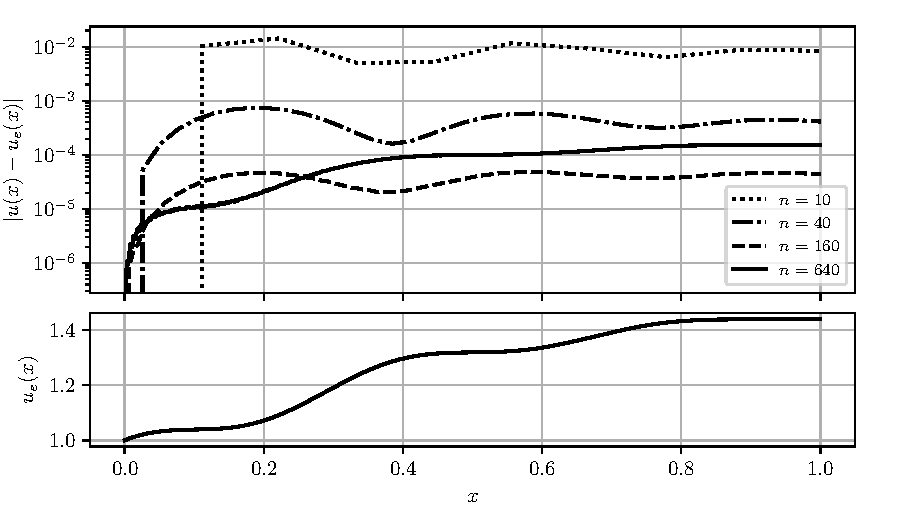
\includegraphics[width=1.0\linewidth]{../images/prob_2_part_c.pdf}
	\caption{The exact solution for \cref{claim_prob_2_part_3} (bottom axes) and the absolute error $| u(x) - u_e(x) |$ (top axes) for an indicated number of degrees of freedom $n$.
	The code used to generate this plot is given in Code \cref{plot_prob_c_code}.}
	\label{fig_prob_2_part_c}
\end{figure}

%===============================================================================
%===============================================================================
\newpage
%===============================================================================
%===============================================================================

\subsection{Implementation}

The interval of the analysis is represented by the \texttt{Topology} class (\cref{topology_header_code,topology_code}), and is used to discretize the domain from $x = 0$ to $x = \ell$ into $n$ sub-intervals.
The \texttt{diffusion} method (\cref{diffusion_header_code,diffusion_code}) utilizes the sparse matrix and linear iterative method implementation introduced in \cref{sec_linear_implementation} to derive approximate solutions to the test cases of \cref{sec_prob_2_part_a,sec_prob_2_part_b,sec_prob_2_part_c}.
The \texttt{Makefile} listed in \cref{makefile} may be used to easily compile all of the simulation scripts listed in \cref{prob_2_code_part_a,prob_2_code_part_b,prob_2_code_part_c}.
Finally, each of these simulations may be compared to identical solutions derived using the finite-element software \fenics by running the provided Python scripts (\cref{prob_2_part_a_python_code,prob_2_part_b_python_code,prob_2_part_c_python_code}).

\subsection{Convergence analysis}

Simulations were performed for $n = 10, 20, 40, 80, 160, 320,$ and $640$ degrees of freedom.
The normalized error $\Vert \rankone{u} - \rankone{u}_e \Vert_2 / n$ roughly follows the theoretical discretization error $h = 1/n^2$ (\cref{fig_convergence}).
However, the error associated with test case (c) (see \cref{sec_prob_2_part_c}) stops improving when $n = 320$ and becomes worse with further mesh refinement.
This may be due to the sharp discontinuity in the conductivity of this simulation at $x = 0.5$ (\cref{fig_prob_2_part_c}).
In addition, the error associated with test case (a) (see \cref{sec_prob_2_part_a}) is always minimal (\cref{fig_convergence}).
In fact, it can be shown that the solution is exact at each of the inter-element nodes (see Appendix H of \citet{zienkiewicz_2000}).
Therefore, the error indicated in \cref{fig_prob_2_part_a,fig_convergence} is due solely to the error induced by using an iterative method (see \cref{def_forward_gauss}).


\begin{figure}
	\centering
		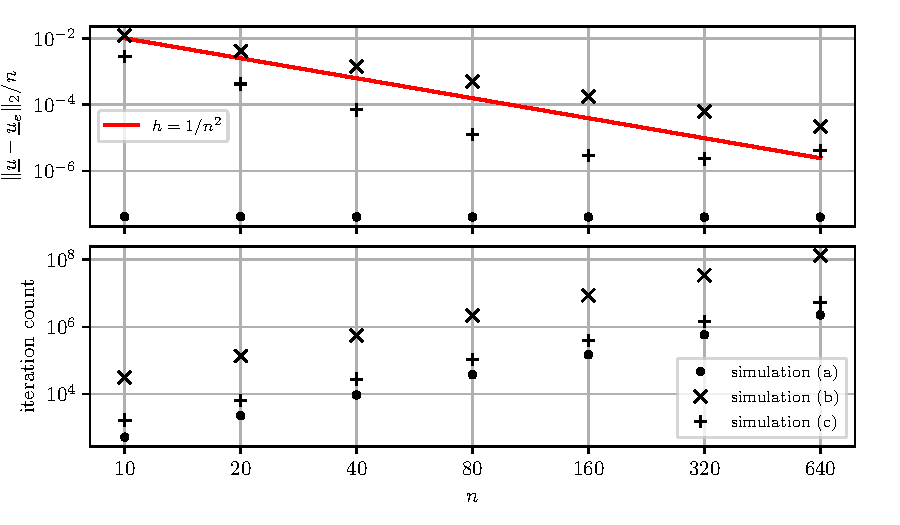
\includegraphics[width=1.0\linewidth]{../images/prob_2_convergence.pdf}
	\caption{The normalized error $\Vert \rankone{u} - \rankone{u}_e \Vert_2 / n$ (top axes) and iteration count (bottom axes) for a given number of degrees of freedom $n$.
	The theoretical convergence rate of the discretization (top figure, solid line) is given for comparison.
	The code used to generate this plot is given in Code \cref{iteration_plot_code}.}
	\label{fig_convergence}
\end{figure}

\newpage

\subsection{Source code}

\pythonexternal[label={makefile}, caption={Makefile which may be used to compile the source code.}]{../simulations/Makefile}

\newpage

\cppexternal[label={topology_header_code}, caption={C++ header file for a topological space with implementation \cref{topology_code}.}]{../src/topology.h}

\newpage

\cppexternal[label={topology_code}, caption={C++ source code for a topological space.}]{../src/topology.cpp}

\newpage

\cppexternal[label={diffusion_header_code}, caption={C++ header file for diffusion solution methods with implementation \cref{diffusion_code}.}]{../src/diffusion.h}

\newpage

\cppexternal[label={diffusion_code}, caption={C++ source code for the diffusion solution methods.}]{../src/diffusion.cpp}

\newpage

\cppexternal[label={prob_2_code_part_a}, caption={C++ source code used solve Problem 2 \cref{sec_prob_2_part_a} utilizing the linear solver defined in \cref{linear_code}.}]{../simulations/prob_2_part_a.cpp}

\newpage

\cppexternal[label={prob_2_code_part_b}, caption={C++ source code used solve Problem 2 \cref{sec_prob_2_part_b} utilizing the linear solver defined in \cref{linear_code}.}]{../simulations/prob_2_part_b.cpp}

\newpage

\cppexternal[label={prob_2_code_part_c}, caption={C++ source code used solve Problem 2 \cref{sec_prob_2_part_c} utilizing the linear solver defined in \cref{linear_code}.}]{../simulations/prob_2_part_c.cpp}

\newpage

\pythonexternal[label={prob_2_part_a_python_code}, caption={Python source code used solve Problem 2 \cref{sec_prob_2_part_a} utilizing \fenics.}]{../fenics/prob_2_part_a.py}

\pythonexternal[label={prob_2_part_b_python_code}, caption={Python source code used solve Problem 2 \cref{sec_prob_2_part_b} utilizing \fenics.}]{../fenics/prob_2_part_b.py}

\pythonexternal[label={prob_2_part_c_python_code}, caption={Python source code used solve Problem 2 \cref{sec_prob_2_part_c} utilizing \fenics.}]{../fenics/prob_2_part_c.py}

\newpage

\pythonexternal[label={plot_prob_a_code}, caption={Python source code used to generate \cref{fig_prob_2_part_a}.}]{../plotting/plot_prob_2_a.py}

\newpage

\pythonexternal[label={plot_prob_b_code}, caption={Python source code used to generate \cref{fig_prob_2_part_b}.}]{../plotting/plot_prob_2_b.py}

\newpage

\pythonexternal[label={plot_prob_c_code}, caption={Python source code used to generate \cref{fig_prob_2_part_c}.}]{../plotting/plot_prob_2_c.py}

\newpage

\pythonexternal[label={iteration_plot_code}, caption={Python source code used to generate \cref{fig_convergence}.}]{../plotting/plot_iteration.py}

%===============================================================================
%===============================================================================
\newpage
%===============================================================================
%===============================================================================

% here we change the meaning of \VAN to use the prefix for the bibliography
\DeclareRobustCommand{\VAN}[3]{#3}

\printbibliography

\end{document}



